\documentclass{article}
\input{/Users/joshyv/Research/misc/my_latex_defs.tex}
\begin{document}

\paragraph{major revisions}

\begin{enumerate}
\item indicate throughout that we are dealing with a time-series, not the raw fluorescence movies
\item stop using the word ``intermittent'', and replace it with superresolution (which sets up a nice parallel in terms of Abbe's limit and the Nyquist sampling theorem)
\item briefly explain general smc-em in text (ie, like 1-2 pages --- unlike the current 6 page behomoth we have now), and move the behomoth to the appendix
\item in describing the stuff, start out with the simple vanilla case, ie, no stimulus, no intermittency; then add intermittency, then stimulus, then 1 spike history term (but mention the possibility of more)
\item note that this means that we first explain the conditional sampler assuming we have every observation.  when we add intermittency, we can briefly describe in the main text that we are sampling now according to $P(F_v | C_t)$, where $v>t$, and relegate the details to the appendix.
\item note how this would change the figs (see the proposed new ones for the simulations), which of course requires changes in the results section of the text
\item add a data fig, comparing wiener, pf not using stimulus, and pf using stimulus
\item these proposed changes would also mean that the other figs should be modified somewhat
\end{enumerate}


\paragraph{minor revisions}


\begin{enumerate}
\item change title to: Model-based inference of spike times given noisy and temporally subsampled calcium-sensitive fluorescence time-series
\item add bruno to author list
\item generall replace ``fluorescence'' with ``intensity'' to be more generally inclusive of ratiometric, and non-fluorescent images (eg, SHG)
\item abstract: replace ``variances'' with ``errorbars''
\item note that we assume we have been given a time-series
\item keywords: replace ``undersample'' with ``temporally subsample''
\item combine epi and confocal sentences
\item add holy ref in intro 
\item last line of pg. 2, add ``(though see Borst and Abarbanel, 2007)''
\item change ``dt'' to $\Delta$ to avoid confusion with an integral
\item acknowledge in ``Model'' section that intermittent observations may come from camera malfunction, or other weird stuff
\item change $\alpha$ and $\beta$ to $F_{max}$ and $F_min$
\item fix up discussion about intermittent using 2p vs. epi
\item in discussion of noise, mention work in progress on spatiotemporal filtering of raw movie data
\item mention SHG after eq (2)
\item in discussion of Ca dynamics
\item change $\tau_c$ and $\sigma_c$ to simply $\tau$ and $\sigma$
\item reword the sentence before eqs (7) and (8)
\item i dropped $_{Tr}$ subscript in eq (24)
\item pg 13 has a $p(F_v|[$Ca$^{2+}]_v)$, which should be $P_{\vec{\theta}}(\cdot)$ 
\item eqs (31) and (32) should explicitly write posterior% instead of $M_t^{(i)$
\item remove ``our'' from from summary paragraph 
\end{enumerate}


\paragraph{stuff i did}

\begin{enumerate}
\item removed ``soma, dendrite, etc.'' discussion from methods
\item removed ``fluorescence, FRET, etc. discussion
\end{enumerate}

\includegraphics{~/Research/code/fast_code/SaturSim}
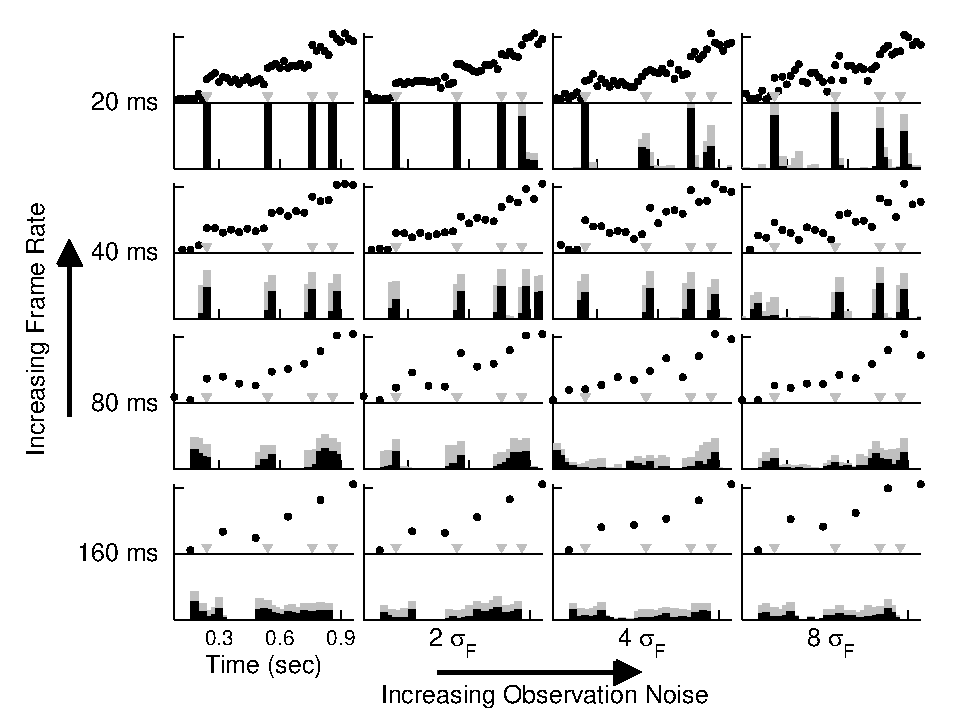
\includegraphics{~/Research/code/fast_code/ArraySim}
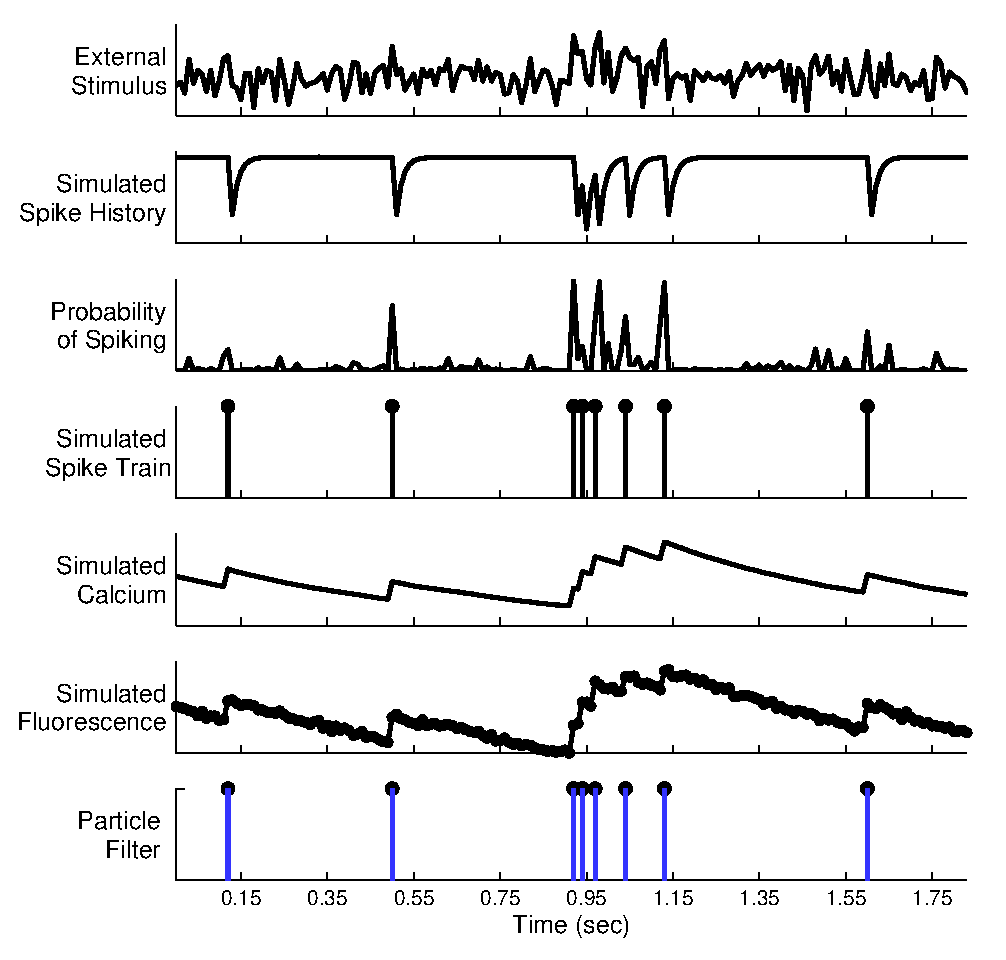
\includegraphics{StimSim}
\includegraphics{KernelSim}


\end{document}
